
%Photo des opérateurs
%\begin{figure}[!h]
%    \centering
%    \begin{subfigure}[b]{0.45\textwidth}
%        \includegraphics[angle=0,viewport=0 0 1600 1200,bb=0 0 4000 3000,width=6.6cm,keepaspectratio=true]{P1020548.JPG}
%        \caption{?}%+200+150
%        \label{P1020548}
%    \end{subfigure}
%    ~
%    \begin{subfigure}[b]{0.45\textwidth}
%        \includegraphics[angle=0,viewport=0 0 1600 1200,bb=0 0 4000 3000,width=6.6cm,keepaspectratio=true]{P1020549.JPG}
%        \caption{?}%+200+150
%        \label{P1020549}
%    \end{subfigure}
%    \caption{Observations à partir de la Station 1}
%    \label{Points Cibles S1}
%\end{figure}


\section{Les Points cibles}

\subsection{Station 1}
\begin{figure}[!h]
    \centering
    \begin{subfigure}[b]{0.3\textwidth}
        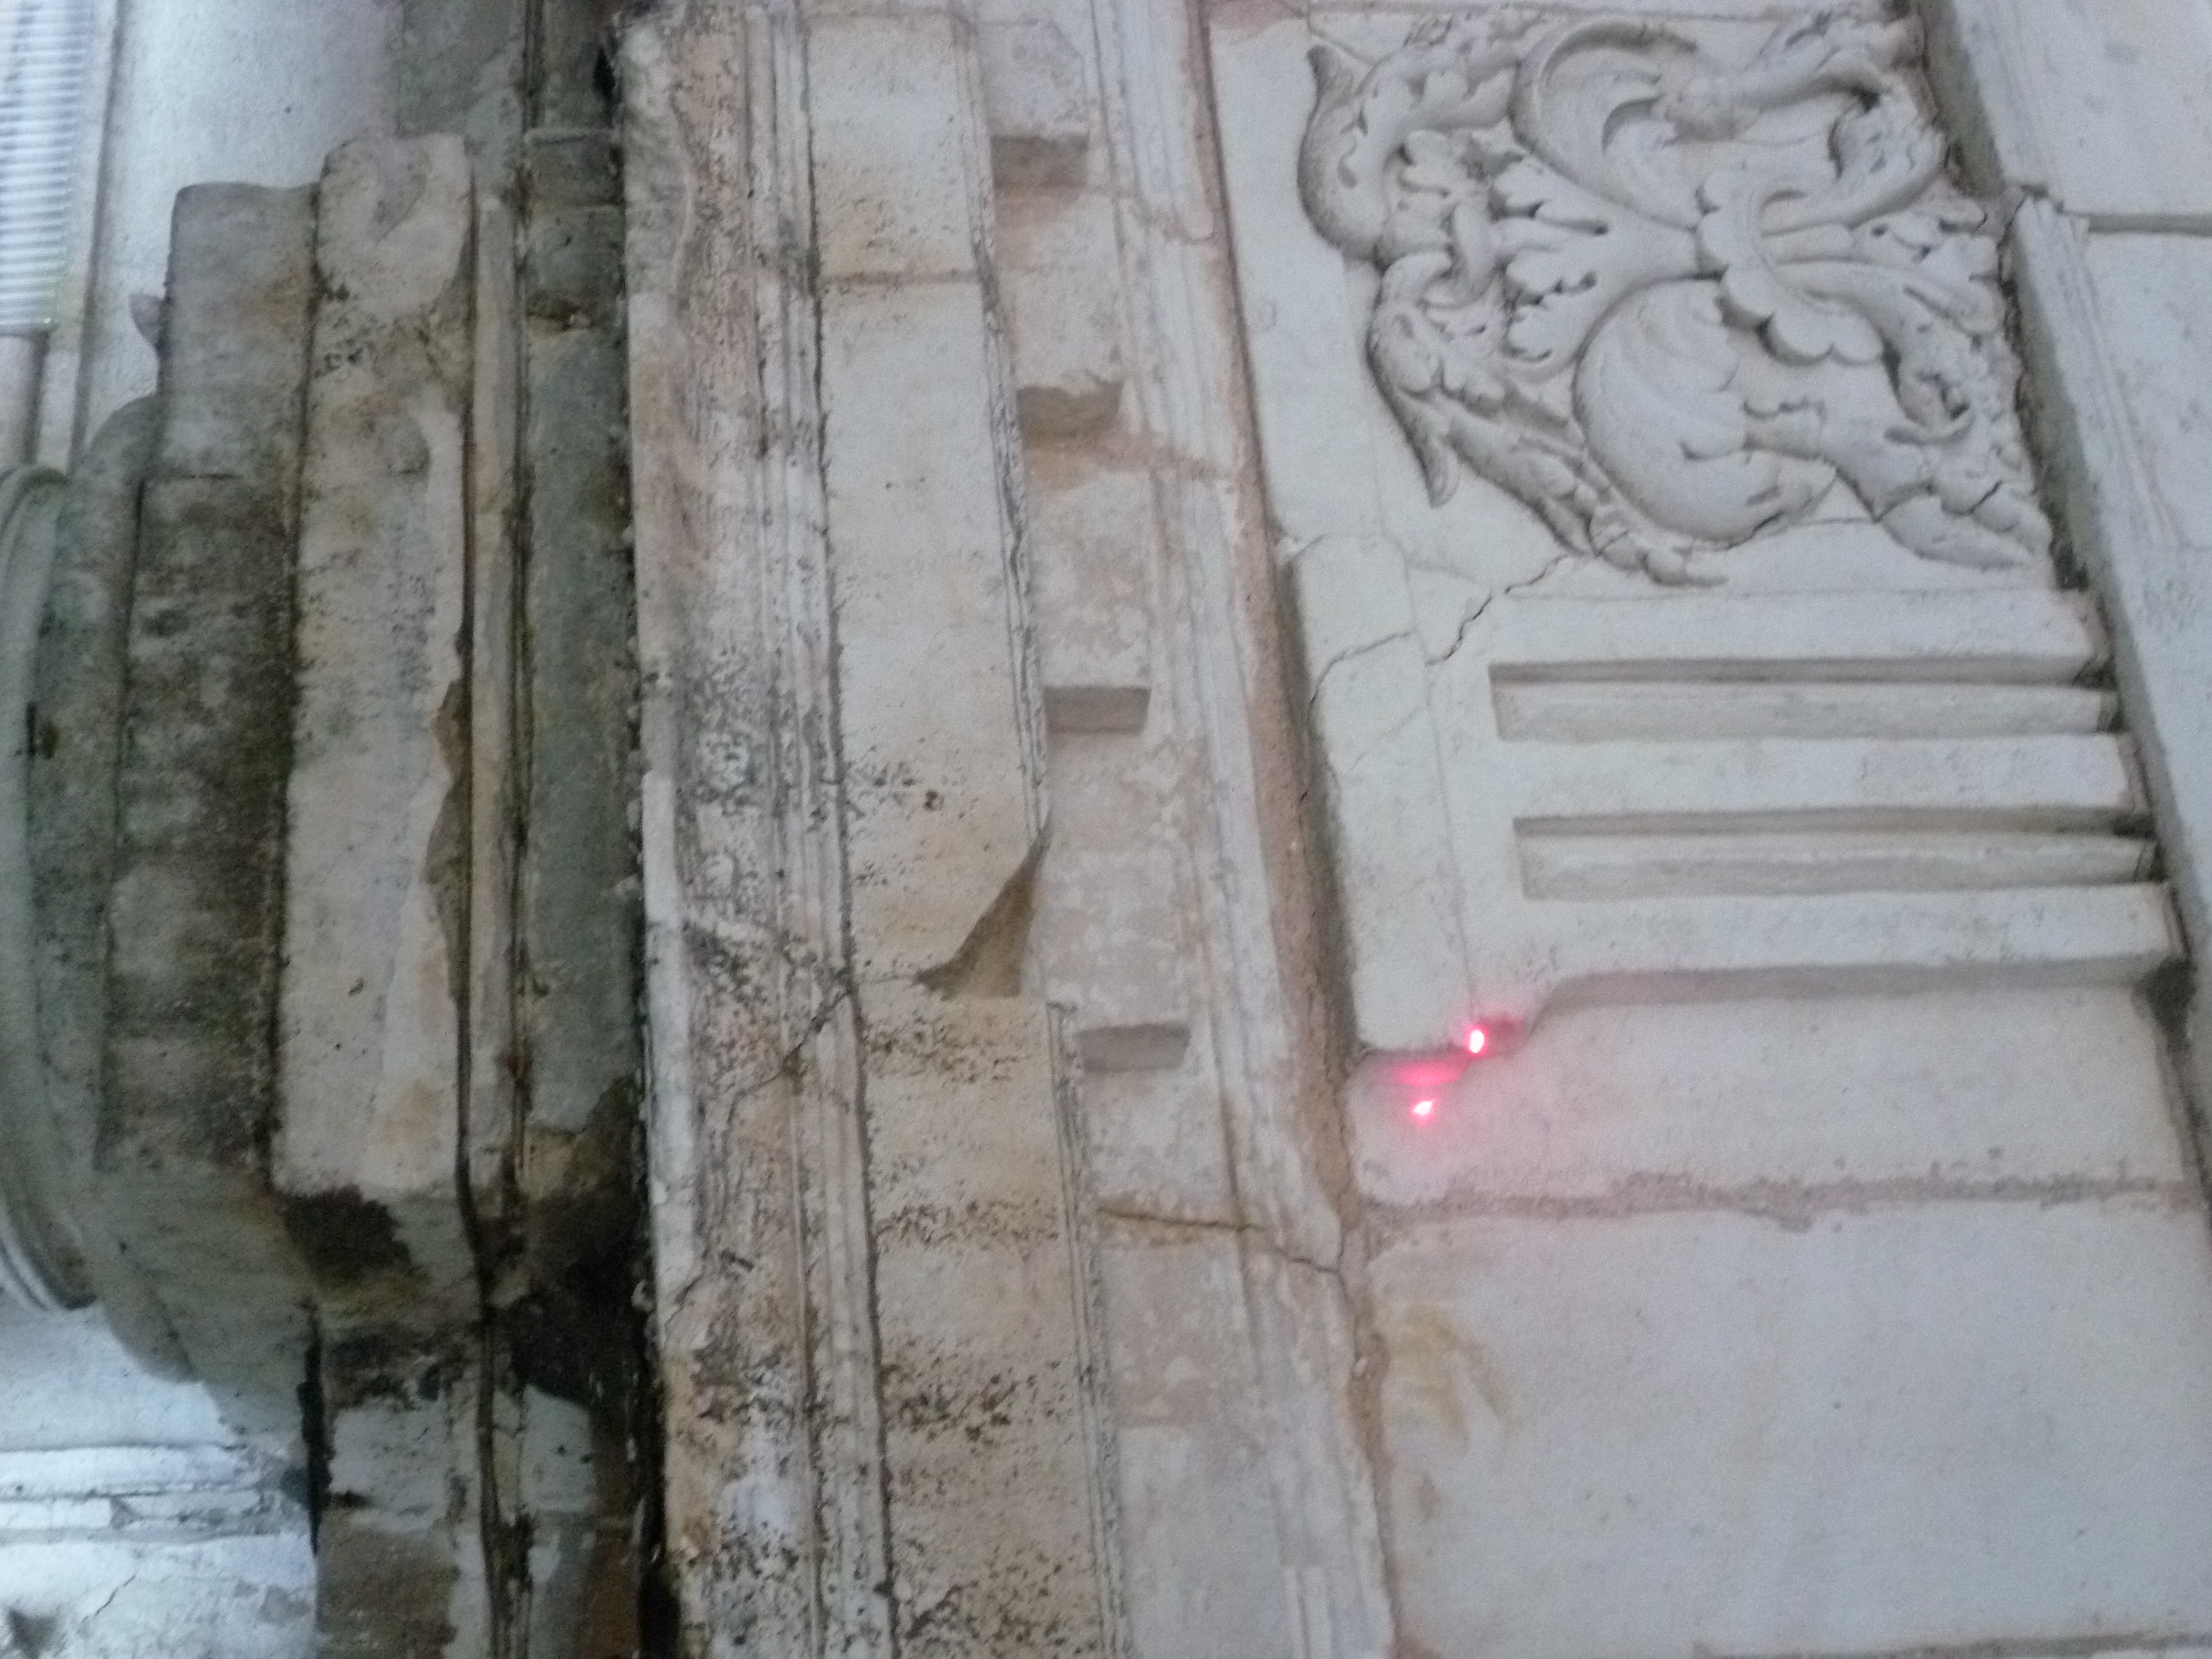
\includegraphics[angle=-90,viewport=0 0 1600 1200,bb=0 0 4000 3000,width=3.3cm,keepaspectratio=true]{P1020538.JPG}
        \caption{1009}%+200+150
        \label{P1020538}
    \end{subfigure}
    ~
    \begin{subfigure}[b]{0.3\textwidth}
        \includegraphics[angle=0,viewport=0 0 1600 1200,bb=0 0 4000 3000,width=4.4cm,keepaspectratio=true]{P1020539.JPG}
        \caption{1010}%+200+150
        \label{P1020539}
    \end{subfigure}
    ~
    \begin{subfigure}[b]{0.3\textwidth}
        \includegraphics[angle=0,viewport=0 0 1600 1200,bb=0 0 4000 3000,width=4.4cm,keepaspectratio=true]{P1020540.JPG}
        \caption{1011}%+200+150
        \label{P1020540}
    \end{subfigure}
    \\
    \begin{subfigure}[b]{0.3\textwidth}
        \includegraphics[angle=0,viewport=0 0 1600 1200,bb=0 0 4000 3000,width=4.4cm,keepaspectratio=true]{P1020541.JPG}
        \caption{1012}%+200+150
        \label{P1020541}
    \end{subfigure}
    ~
    \begin{subfigure}[b]{0.3\textwidth}
        \includegraphics[angle=0,viewport=0 0 1600 1200,bb=0 0 4000 3000,width=4.4cm,keepaspectratio=true]{P1020542.JPG}
        \caption{1013}%+200+150
        \label{P1020542}
    \end{subfigure}
    ~
    \begin{subfigure}[b]{0.3\textwidth}
        \includegraphics[angle=0,viewport=0 0 1600 1200,bb=0 0 4000 3000,width=4.4cm,keepaspectratio=true]{P1020543.JPG}
        \caption{1014}%+200+150
        \label{P1020543}
    \end{subfigure}
    \caption{Points visés à partir de la Station 1}
    \label{Points Cibles S1a}
\end{figure}

\begin{figure}[!h]
    \centering
    \begin{subfigure}[b]{0.3\textwidth}
        \includegraphics[angle=0,viewport=0 0 1600 1200,bb=0 0 4000 3000,width=4.4cm,keepaspectratio=true]{P1020544.JPG}
        \caption{1015}%+200+150
        \label{P1020544}
    \end{subfigure}
    ~
    \begin{subfigure}[b]{0.3\textwidth}
        \includegraphics[angle=0,viewport=0 0 1600 1200,bb=0 0 4000 3000,width=4.4cm,keepaspectratio=true]{P1020545.JPG}
        \caption{1016}%+200+150
        \label{P1020545}
    \end{subfigure}
    ~
    \begin{subfigure}[b]{0.3\textwidth}
        \includegraphics[angle=0,viewport=0 0 1600 1200,bb=0 0 4000 3000,width=4.4cm,keepaspectratio=true]{P1020547.JPG}
        \caption{1017}%+200+150
        \label{P1020547}
    \end{subfigure}
    \caption{Suite des points visés à partir de la Station 1}
    \label{Points Cibles S1b}
\end{figure}

% detail des points
\includePhotoDetailVerticalDixQuatre{P1020538}{1009}
\includePhotoDetailHorizontalHuitSix{P1020539}{1010}%{0}
\includePhotoDetailHorizontalHuitHuit{P1020540}{1011}
\includePhotoDetailHorizontalHuitSix{P1020541}{1012}
\includePhotoDetailHorizontalHuitSix{P1020542}{1013}
\includePhotoDetailHorizontalHuitHuit{P1020543}{1014}
\includePhotoDetailHorizontalHuitHuit{P1020544}{1015}
\includePhotoDetailHorizontalHuitSix{P1020545}{1016}
\includePhotoDetailHorizontalHuitSix{P1020547}{1017}

%Détail du point 1016

\subsection{Station 2}
\begin{figure}[!h]
    \centering
    \begin{subfigure}[b]{0.3\textwidth}
        \includegraphics[angle=-90,viewport=0 0 1600 1200,bb=0 0 4000 3000,width=3.3cm,keepaspectratio=true]{P1020563.JPG}
        \caption{1024}%+200+150
        \label{P1020563}
    \end{subfigure}
    ~
    \begin{subfigure}[b]{0.3\textwidth}
        \includegraphics[angle=0,viewport=0 0 1600 1200,bb=0 0 4000 3000,width=4.4cm,keepaspectratio=true]{P1020564.JPG}
        \caption{1025}%+200+150
        \label{P1020564}
    \end{subfigure}
    ~
    \begin{subfigure}[b]{0.3\textwidth}
        \includegraphics[angle=0,viewport=0 0 1600 1200,bb=0 0 4000 3000,width=4.4cm,keepaspectratio=true]{P1020565.JPG}
        \caption{1026}%+200+150
        \label{P1020565}
    \end{subfigure}
    \\
    \begin{subfigure}[b]{0.3\textwidth}
        \includegraphics[angle=0,viewport=0 0 1600 1200,bb=0 0 4000 3000,width=4.4cm,keepaspectratio=true]{P1020566.JPG}
        \caption{1027}%+200+150
        \label{P1020566}
    \end{subfigure}
    ~
    \begin{subfigure}[b]{0.3\textwidth}
        \includegraphics[angle=0,viewport=0 0 1600 1200,bb=0 0 4000 3000,width=4.4cm,keepaspectratio=true]{P1020567.JPG}
        \caption{1028}%+200+150
        \label{P1020567}
    \end{subfigure}
    ~
    \begin{subfigure}[b]{0.3\textwidth}
        \includegraphics[angle=0,viewport=0 0 1600 1200,bb=0 0 4000 3000,width=4.4cm,keepaspectratio=true]{P1020568.JPG}
        \caption{1029}%+200+150
        \label{P1020568}
    \end{subfigure}
    \caption{Points visés à partir de la Station 2}
    \label{Points Cibles S2a}
\end{figure}
\begin{figure}[!h]
    \centering
    \begin{subfigure}[b]{0.3\textwidth}
        \includegraphics[angle=-90,viewport=0 0 1600 1200,bb=0 0 4000 3000,width=3.3cm,keepaspectratio=true]{P1020569.JPG}
        \caption{1030}%+200+150
        \label{P1020569}
    \end{subfigure}
    ~
    \begin{subfigure}[b]{0.3\textwidth}
        \includegraphics[angle=0,viewport=0 0 1600 1200,bb=0 0 4000 3000,width=4.4cm,keepaspectratio=true]{P1020570.JPG}
        \caption{1031}%+200+150
        \label{P1020570}
    \end{subfigure}
    ~
    \begin{subfigure}[b]{0.3\textwidth}
        \includegraphics[angle=0,viewport=0 0 1600 1200,bb=0 0 4000 3000,width=4.4cm,keepaspectratio=true]{P1020572.JPG}
        \caption{1032}%+200+150
        \label{P1020572}
    \end{subfigure}
    \\
    \begin{subfigure}[b]{0.3\textwidth}
        \includegraphics[angle=0,viewport=0 0 1600 1200,bb=0 0 4000 3000,width=4.4cm,keepaspectratio=true]{P1020573.JPG}
        \caption{1033}%+200+150
        \label{P1020573}
    \end{subfigure}
    ~
    \begin{subfigure}[b]{0.3\textwidth}
        \includegraphics[angle=0,viewport=0 0 1600 1200,bb=0 0 4000 3000,width=4.4cm,keepaspectratio=true]{P1020574.JPG}
        \caption{1034}%+200+150
        \label{P1020574}
    \end{subfigure}
    ~
    \begin{subfigure}[b]{0.3\textwidth}
        \includegraphics[angle=0,viewport=0 0 1600 1200,bb=0 0 4000 3000,width=4.4cm,keepaspectratio=true]{P1020575.JPG}
        \caption{1035}%+200+150
        \label{P1020575}
    \end{subfigure}
    \caption{Suite des points visés à partir de la Station 2}
    \label{Points Cibles S2b}
\end{figure}

\includePhotoDetailHorizontalHuitSix{P1020563}{1024}
\includePhotoDetailHorizontalHuitSix{P1020564}{1025}
